\section{Theorie}
In dem verwendeten Aufbau wurden Photonen zur Elektronenanregung verwendet. \\
Wird ein hochenergetisches Photon von einem  kernnahen Elektron des Atoms absorbiert, so wird das Photon vernichtet und das Elektron angeregt. \\
Wobei die Elektronen nur in freie Zustände angeregt werden können. \\
Die Röntgenfluoreszenz entsteht, wenn durch das Photon ein Elektron aus einer inneren Schale angeregt wird und somit einen freien Zustand in dieser Schale zurück lässt. \\
Wodurch ein Elektron aus den äußeren Schalen in den freien Zustand übergehen kann, hauptsächlich durch spontane Emission, wobei ein Photon mit der Energie: \\

\begin{align}
    h f = E_{1} - E_{2}
\end{align}
entstehen kann.\\

Die Energiedifferenz ist elementabhängig, genau wie die Übergangswahrscheinlichkeiten und Anzahl der möglichen Übergänge.
Die Energie kann unter anderem auch als ein Auger-Elektron abgegeben werden. Da wir jedoch nur Photonen, detektieren werden diese Auger-Elektronen nicht weiter betrachtet.\\
\subsection{Fermis Goldene Regel}
Nicht jeder Übergang der Elektronen ist gleich wahrscheinlich oder überhaupt möglich. \\

\begin{align}
    \lambda_{i\rightarrow f} = \frac{2 \pi}{\hB{h}}\rho(E_{f}) \vert V_{f i} \vert ^{2}
\label{Eq:Fermi}
\end{align}

$\lambda_{i\rightarrow f} := $ Übergangswahrscheinlichkeit\\
$\rho(E_{f}):= $ Zustandsdichte \\
$\vert V_{f i} \vert := $ Matrixelement \\ 
Das Matrixelement kann als Dipol-Matrix genähert werden, außerdem muss die Energieerhaltung gegeben sein, weshalb wir die Formel \ref{Eq:Fermi} mit der Formel \ref{Eq:Nahrung} näheren können.
\begin{align}
\label{Eq:Nahrung}
\lambda_{i\rightarrow f} \propto <f \vert r \cdot \epsilon \vert i > \delta ( E_{f} - E_{i} - hf) \rho(E_{f})
\end{align}
Aus dem Dipolmatrixelement lassen sich Auswahlregeln ableiten welche Übergänge möglich sind.
Der Elektronenspin muss identisch sein so das $ \Delta s= 0 $
gilt. Da das Photon den Elektronenspin nicht beeinflusst. Zudem muss der Bahndrehimpuls erhalten bleiben wodurch sich die Voraussetzung $ \Delta l = \pm 1 $  ergibt.
Sowie für den Gesamtdrehimpuls gelten muss: $\Delta j = 0,\pm1 $ \\
Ein Beispiel ist der $K_{\alpha 1}$ Übergang bei dem ein Elektron aus der N-Schale in die K-Schale übergeht.\\
Quantenmeschanisch ist das ein Übergang von:\\ $L_{3}(2p_{3/2}) \rightarrow K(1s)$

\subsection{Röntgenröhre}
Bei der Röntgenröhre werden Elektronen aus einer vorgeheizten Kathode heraus gelöst. Durch die Beschleunigungsspannung $U_\text{B}$ werden die Elektronen von der Kathode zur Anode beschleunigt,
\begin{equation*}E_\text{kin} = U_\text{B} \cdot e\end{equation*}
treffen auf die Anode auf und werden entweder abgebremst oder stoßen mit weiteren Elektronen in der Anode, siehe Abb. \ref{fig:röntgenröhre}.
Die abgebremsten Elektronen verursachen ein kontinuierliches Spektrum, welches Bremsspektrum genannt wird, siehe Abb. \ref{fig:bremsspektrum}. Die minimale Wellenlänge ist die, bei der die gesamte kinetische Energie in die Energie des Photons umgewandelt wurde.
\begin{equation*}E_\text{kin} = \frac{hc}{\lambda}\end{equation*}
\begin{figure}[H]
\begin{minipage}{0.5\textwidth}
    \centering
    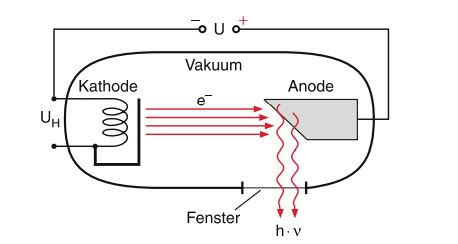
\includegraphics[width=0.9\textwidth]{Röntgen.JPG}
    \caption[Funktionsprinzip Röntgenröhre]{Schematische Darstellung des Funktionsprinzips einer Röntgenröhre \cite{demtroder3}.}
    \label{fig:röntgenröhre}
\end{minipage}\hfill
\begin{minipage}{0.5\textwidth}
    \centering
    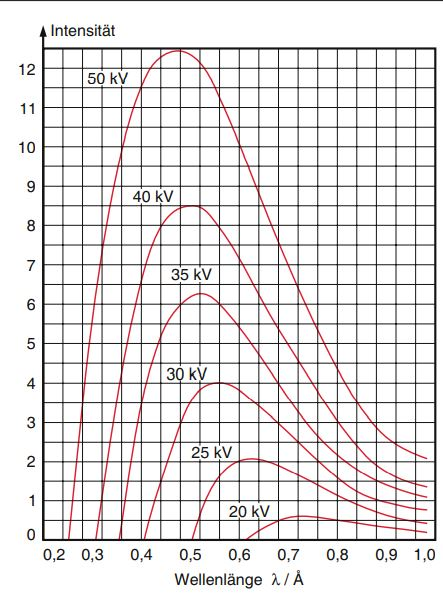
\includegraphics[width=0.8\textwidth]{bremse.JPG}
    \caption[Bremsspektren]{Darstellung verschiedener Bremsspektren. Die Intensität ist über der Wellenlänge aufgetragen \cite{demtroder3}.}
    \label{fig:bremsspektrum}
\end{minipage}
\end{figure}
Durch die inelastischen Stöße werden tief liegende Elektronen heraus geschlagen. Ein energetisch höher liegendes Elektron rückt nach, wodurch ein Photon emittiert wird mit der Energie:
\begin{equation*}E = E_2 - E_1 = hf\end{equation*}
Es kommt zur Abstrahlung von Strahlung mit charakteristischen Wellenlängen. Die Überlagerung der Bremsstrahlung und der charakteristischen Strahlung ergibt das Spektrum der Röntgenanode, siehe Abb. \ref{fig:röntgenspektrum}.
\begin{figure}[H]
\centering
    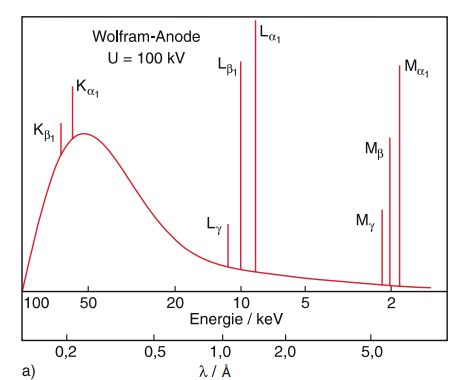
\includegraphics[width=0.5\textwidth]{spektrum.JPG}
    \caption[Röntgenspektrum]{Charakteristisches Röntgenspektrum \cite{demtroder3}.}
    \label{fig:röntgenspektrum}
\end{figure}


\subsection{Photonenstreuung}
Zwei häufig auftretende Streuprozesse ist die elastische  Rayleigh-Streuung un die inelastische Compton-Streuung.  
Das Verhältniss von elastisch und inelastischer Streuung ist grob abhängig von der Massezahl des zu unterschenden Elements. Bei hohen Massezahlen ist die eleastische Streung deutlich wahrscheinlicher und bei leichten Elementen ist die inelastische Streung wahrscheinlicher. 
\subsubsection{Rayleigh Streung}
Bei der Rayleigh-Streuung werden die Photonen an gebunden Elektronen elastisch gestreut. Was bedeutet das die Energie des Photons unverändert bleibt.\\
Der Wirkungsquerschnitt der Elektronen ist dabei stark Wellenlängenabhängig.\\
Streuqerschnitt:\\
\begin{align}
    \sigma = \frac{8 \pi }{3}r_{e}^2 \frac{\omega^4}{(\omega -\omega_{s}^2)^2+(\gamma \omega)^2}
\end{align}
$\omega :=$ Lichtfrequenz \\
$w_{s} :=$ Resonanzfrequenz \\
$\gamma :=$ Dämpfung \\
$r_{e} :=$ Semiklassicher Elektronenradius \\
%\begin{figure}[h]
 %\centering
 %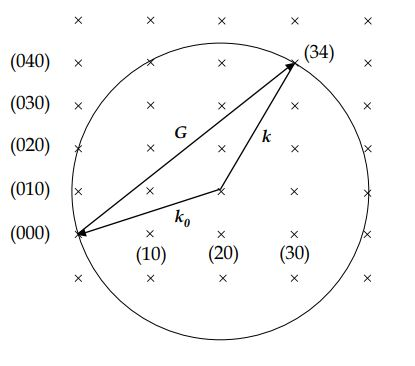
\includegraphics[width=0.7\textwidth]{Bragg.JPG}
 %\caption[Bragg-Bedingung]{Abgebildet ist eine Ewand-Kugel im Reziproken Gitter, zur Darstellung der Bragg-Bedingung \cite{bib:Bragg} }
 %\label{fig:bragg}
%\end{figure}
\subsubsection{Compton-Streuung}
Unter anderem können die Photonen inelastisch an quasi freien Elektronen streuen, diese Peaks zeichnen sich durch ihre große Breite aus. Es handelt sich um Compton-Streuung.
Die Energieänderung der Photonen lässt sich durch die inelastische Streuung mit den Elektronen mit der allgemein bekannten Compton-Formel beschreiben.
\begin{align}
\label{eq:Compton}
h\nu_{0}-h\nu = h \nu_{0} \frac{\lambda(1-cos\theta)}{1+ \lambda(1-cos \theta)}
\end{align}

\subsection{Siliziumdriftdetektor}
\begin{figure}[h]
 \centering
 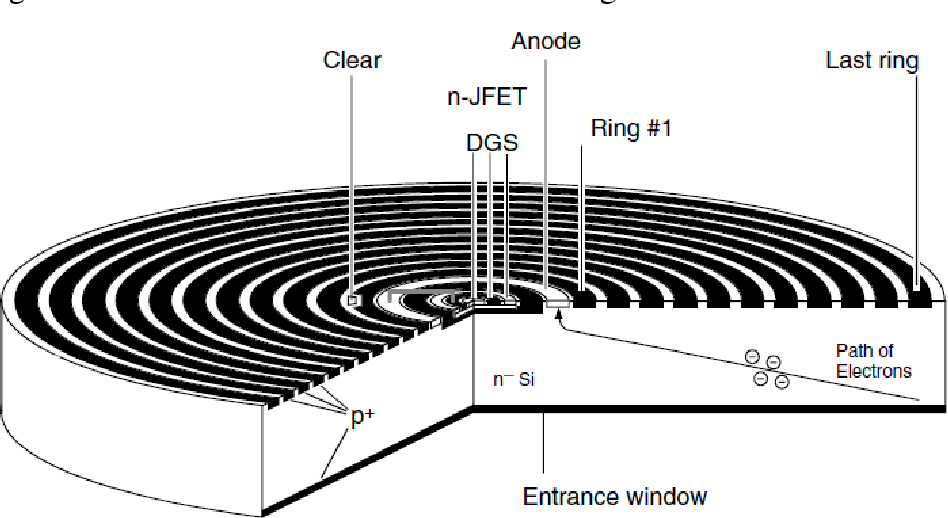
\includegraphics[width=0.7\textwidth]{SSD.png}
 \caption[SDD]{Abgebildet ist eine schematische Darstellung des SDD. \cite{bib:SDD}}
 \label{fig:SDD}
\end{figure}
Algemein dient der Siliziumdriftdetektor, im folgendem SDD genannt, zur energiedispersiven Messung ionisierender Strahlung.
Er besteht aus einem PN-Übergang.
Wobei der P-Leiter, in der Abbildung \ref{fig:SDD} schwarz dargestellt,  eine deutlich höhere Dotierkonzentration besitzt als der N-Leiter. Somit ist die Verarmungszone weit in  N-Leiter ausgedehnt.
In der Abbildung \ref{fig:SDD} ist der N-Leiter weiß dargestellt.\\
Moderne SDD haben Ringförmige P-Kontakte auf der Rückseite des Detektors. 

Fällt nun ein Photonen auf den SDD so kann es von einem Elektron absorbiert werden welches dann auf dem Weg durch die Verarmungszone weitere Elektronen in das Leitungsband anregt, und somit Elektronen-Loch-Paare bildet.
Durch die hohe Spannung die an dem SDD anliegt können diese Elektonen-Loch-Paare als Strom detektiert werden. Hierbei ist der Strom proportional zur Photonenenergie. \\
\subsubsection{Detektorartefakte }
Fallen zwei Photonen innerhalb einer kurzen Zeit hintereinander auf den Detektor so kann es passieren dass der Detektor die Photonenenergie addiert und die beiden Photonen als ein Photon zählt, dies wird auch "pille-up" genannt. Beispielsweise ist in Abbildung \ref{fig:Stahlprobe} gut zusehen das der Eisenübergang bei 6keV mit der hohen Zählrate zu einem weiteren Peak bei ca. 12keV führt.
Dies geschieht besonders wahrscheinlich für Photonenenergien die häufig auftreten. 
Escape Peaks entstehen in dem Fall das, ein Röntgenphoton in dem Siliziumkristall des Detektors ein Elektron aus der K-Schale anregt. Das so erzeugte Elektron hat dementsprechend eine um die Ionisationsenergie verringerte Kinetische Energie. 
Das Photon, was durch Relaxation eines energetisch höher liegenden Elektrons entsteht, tritt mit einer gewissen Wahrscheinlichkeit ohne mit dem Detektor zu interagieren, aus dem Siliziumkristalles aus. 
Wodurch auch die vom Detektor suggeriert Energie um die Ionisationsenergie(1,74 keV) niedriger ausfällt.
\subsection{Bragg-Spiegel}
Der Bragg-Spiegel wird genutzt um für eine bestimmte Wellenlänge eine hohe Reflektivität zu erhalten.
Der Bragg-Spiegel besteht aus mehreren Schichten mit abwechselnd optisch dichterem und optisch dünnerem Medium.\\
An jeder Grenzschicht wird ein Teil des Lichts reflektiert.\\
Damit das refektierte Licht konstruktiv interferiert, muss das Licht um ganzzahlige Vielfache der Wellenlänge verzögert sein. Da an jeder Grenzschicht von dem optisch dünnerem zum dichterem Medium ein $\lambda/2$ Phasensprung stattfindet muss die optische dicke der einzelnen Schichten $\lambda/4$ entsprechen. So das die Formel \ref{Eq:Spiegel} erfüllt ist.\\
\begin{align}
    2n_{L}d_{L}+\frac {\lambda }{2}=2n_{H}d_{H}+\frac{\lambda }{2}=m \lambda 
    \label{Eq:Spiegel}
\end{align}


\subsection{Absorptionsfilter}
Um das Anregungsspektrum zu beeinflussen können Absorptionsfilter in verschiedenen Dicken und Materialien gewählt werden.\\
Die Anregungsstrahlung transmitiert durch die Filterblende, in der unter anderem Photonen absorbiert werden können. Daraus bildet sich ein charakteristisches Spektrum mit materialabhängigen Absorbitionskanten. Eine Beispielhafte Absorptionskante ist in Abbildung \ref{fig:Kante} dargestellt.\\
\begin{figure}[h]
 \centering
 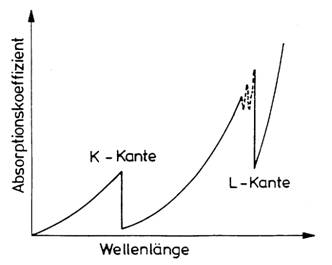
\includegraphics[width=0.7\textwidth]{roentgenabsorption.jpg}
 \caption[Absortionskante]{Absorbtionsspektrum mit Absorbtionskante \cite{bib:Kante} }
 \label{fig:Kante}
\end{figure}
